\subsubsection{Logical Gates}\label{sec:logical-gates}

Originally, before Quantum Error Correction Codes (QECCs), life was easy: physical qubit, apply gate (e.g., Hadamard), get result. After QECC, things are different. A logical qubit is encoded into many physical qubits, and now the question is: ``\emph{how do we apply a gate to the logical qubit if the logical qubit is spread across many physical qubits?}''.

\highspace
\begin{flushleft}
    \textcolor{Green3}{\faIcon{book} \textbf{Logical Gates}}
\end{flushleft}
To apply a gate to a logical qubit, we need to define the gate operation on the logical qubit level. So, each fundamental gate needs to be defined on logical qubits. But the way the logical operation is performed depends on the logical qubit implementation. There is not one universal logical H gate. The implementation depends on the code used to encode the logical qubit.

\highspace
\begin{definitionbox}[: Logical Gate]
    A \definition{Logical Gate} is a quantum \textbf{operation acting on logical qubits}. Since a logical qubit is encoded into multiple physical qubits, a logical gate is implemented through a coordinated sequence of operations on the underlying physical qubits.
\end{definitionbox}

\highspace
\begin{flushleft}
    \textcolor{Green3}{\faIcon{tools} \textbf{Physical Implementation of Logical Gates}}
\end{flushleft}
In superconducting quantum computers, logical gates are ultimately implemented as \textbf{microwave pulses} sent through a cryogenic chip. The physical hardware consists of superconducting circuits, resonators, control lines, and Josephson junctions operating at temperatures close to absolute zero.

\highspace
\textbf{Superconducting qubits} are the most common type of qubit used in current quantum computers (e.g., IBM, Google, Rigetti). The superconducting qubits are typically implemented as cryogenic qubits, which operate at extremely low temperatures $10-20$ millikelvins ($0.01${\textdegree}C above absolute zero, $\approx -273.15${\textdegree}C). At these temperatures, the superconducting materials exhibit almost zero thermal noise, allowing for coherent quantum operations (\autopageref{sec:quantum-computation-errors}). The gates are implemented via microwave pulses that manipulate the energy levels of the superconducting qubits.

\begin{figure}[!htp]
    \centering
    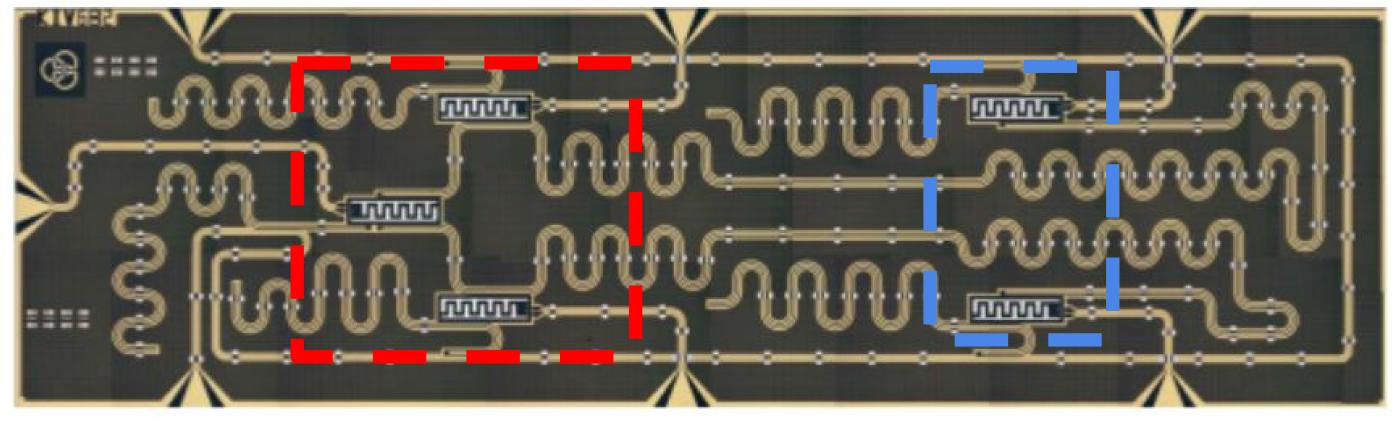
\includegraphics[width=\textwidth]{img/quantum-chip.jpg}
    \caption{Photograph of a \textbf{superconducting quantum chip} used in quantum computing. \cite{quantum-computing-polimi} The squiggly lines are the microwave transmission lines/resonators that control the qubits. The highlighted regions contain the superconducting qubit circuitry and the microwave resonators/control structures used to implement quantum gates through microwave pulses.}
\end{figure}